\vspace{-3pt}
\section{Experimental Results}
\label{sec:experimental_results}

\begin{table*}[t]
\centering
\resizebox{\textwidth}{!}{%
\begin{tabular}{l|cccc|cccc|cccc|cccc}
\toprule
\multirow{2}{*}{\textbf{Methods}} & \multicolumn{4}{c|}{\textbf{MPReID}} & \multicolumn{4}{c|}{\textbf{HMReID}} & \multicolumn{4}{c|}{\textbf{GibsonReID}} & \multicolumn{4}{c}{\textbf{ReplicaReID}} \\
 & Accuracy & Precision & Recall & F1 & Accuracy & Precision & Recall & F1 & Accuracy & Precision & Recall & F1 & Accuracy & Precision & Recall & F1 \\
\midrule
CVNet & 17.45 & 29.52 & 17.45 & 19.34 & 11.71 & 25.42 & 11.95 & 13.86 & 12.04 & 24.06 & 12.07 & 14.27 & 15.93 & 20.53 & 15.74 & 16.64 \\
DINOv2 & 59.36 & 64.68 & 59.36 & 58.91 & 53.91 & 60.52 & 53.73 & 54.69 & 61.01 & 65.88 & 61.78 & 61.71 & 78.06 & 79.68 & 77.97 & 77.44 \\
Patch-NetVLAD & 64.32 & 70.47 & 64.36 & 65.53 & 64.86 & 68.78 & 64.32 & 65.16 & 61.47 & 66.90 & 62.04 & 62.51 & 63.77 & 64.97 & 63.86 & 63.87 \\
AnyLoc & 92.34 & 93.23 & 92.36 & 92.32 & 89.69 & 90.25 & 89.53 & 89.62 & 85.85 & 87.42 & 86.15 & 86.21 & \textbf{88.57} & \textbf{89.89} & \textbf{88.46} & \textbf{88.42} \\
\rowcolor{Lavender}
AirRoom & \textbf{93.96} & \textbf{94.52} & \textbf{93.98} & \textbf{93.91} & \textbf{93.80} & \textbf{94.01} & \textbf{93.55} & \textbf{93.62} & \textbf{91.68} & \textbf{92.41} & \textbf{91.79} & \textbf{91.63} & 87.18 & 89.39 & 87.08 & 87.24 \\
\bottomrule
\end{tabular}%
}
\vspace{-5pt}
\caption{Overall performance comparison between AirRoom and baseline models on four newly constructed room ReID datasets.}
\vspace{-12pt}
\label{tab:overall}
\end{table*}

\subsection{Datasets}
\vspace{-5pt}
No existing indoor scene datasets are ideally suited for room reidentification tasks, as none fully satisfy the requirements.  Datasets like ScanNet++ \cite{yeshwanth2023scannethighfidelitydataset3d} and MIT Indoor Scenes \cite{5206537} lack room-level segmentation, resulting in multiple rooms sharing a single scene label. The 17 Places \cite{7801503} dataset includes uniquely labeled rooms but offers limited viewpoint variations, and the images are often vague. While this dataset also includes day-night changes, these are not particularly relevant for most indoor scenarios. The Reloc110 \cite{aryan2023airlocobjectbasedindoorrelocalization} dataset is likely the most suitable option; however, its quality is insufficient, with many images containing only solid-colored walls or floors due to random sampling, resulting in minimal contextual information.

Several high-quality indoor 3D datasets—such as Matterport3D \cite{Matterport3D}, Habitat-Matterport3D \cite{ramakrishnan2021hm3d}, the Gibson Database of 3D Spaces \cite{xiazamirhe2018gibsonenv}, and Replica \cite{replica19arxiv}—offer real-world indoor scenes. Building on these resources and utilizing the interactive Habitat Simulator \cite{puig2023habitat3, szot2021habitat, habitat19iccv}, we created four new datasets: MPReID, HMReID, GibsonReID, and ReplicaReID, as shown in \fref{fig:dataset_image}.

%Fortunately, several high-quality indoor 3D datasets—such as Matterport3D \cite{Matterport3D}, Habitat-Matterport3D \cite{ramakrishnan2021hm3d}, the Gibson Database of 3D Spaces \cite{xiazamirhe2018gibsonenv}, and Replica \cite{replica19arxiv}—offer real-world scenes, providing a solid foundation for representing indoor environments. Leveraging these resources alongside the interactive Habitat Simulator \cite{puig2023habitat3, szot2021habitat, habitat19iccv}, we developed four new datasets: MPReID, HMReID, GibsonReID, and ReplicaReID, as illustrated in \fref{fig:dataset_image}.

% Utilizing the Habitat Simulator, we configured an agent for each room and manually selected 5 to 10 key poses to guide its exploration. The agent captured 640×480 RGB-D images from various angles, resulting in 300 to 800 images per room, depending on the number of key poses. However, many randomly sampled images were of low quality, often depicting only walls or floors without meaningful context. To address this issue, we carefully filtered the images for each room, retaining only those that accurately represented the space and contributed valuable information for ReID. In total, MPReID includes 15 scenes, 105 rooms, and 16,231 RGB-D images. HMReID consists of 21 scenes, 105 rooms, and 15,781 RGB-D images. GibsonReID features 24 scenes, 45 rooms, and 6743 RGB-D images. ReplicaReID contains 12 scenes, 19 rooms, and 2862 RGB-D images.

Using the Habitat Simulator, we configured an agent for each room and manually selected 5 to 10 key poses to guide its exploration. The agent captured 640×480 RGB-D images from various angles, resulting in 300 to 800 images per room, depending on the number of key poses. However, many randomly sampled images were of low quality, often containing only walls or floors with minimal context. To address this, we carefully filtered the images for each room, retaining those that accurately represented the space and provided valuable information for room ReID.

In total, the datasets are as follows: MPReID includes 15 scenes, 105 rooms, and 16,231 RGB-D images; HMReID consists of 21 scenes, 105 rooms, and 15,781 RGB-D images; GibsonReID contains 24 scenes, 45 rooms, and 6,743 RGB-D images; and ReplicaReID includes 12 scenes, 19 rooms, and 2,862 RGB-D images.


\vspace{-4pt}
\subsection{Database Preprocess}
\vspace{-4pt}

In the room reidentification setting, we have multiple query images and a reference database. For each dataset, we select only one image per room to build the database. Specifically, for all the images of each room, we first use CLIP \cite{radford2021learningtransferablevisualmodels} to extract feature embeddings. Then, we apply K-means clustering with the number of clusters set to 1. The image closest to the cluster center is chosen as the reference image, as it best represents the room's visual characteristics \cite{tan2005introduction}.

After building the reference database, we preprocess features. First, we use the Global Feature Extractor to obtain and save the global context features. Next, we apply the instance segmentation module to segment the objects. Then, we use our Receptive Field Expander to obtain object patches and the Object Feature Extractor to extract and save the features of both the objects and the patches.


\vspace{-4pt}
\subsection{Experimental Overview}
\vspace{-4pt}
We conducted five primary experiments: overall performance comparison, group-wise performance comparison, pipeline flexibility evaluation, ablation studies, and runtime analysis. For evaluation, we used accuracy, precision, recall, and the F1 score as metrics. Per-class precision, recall, and F1-score were computed using a multi-class confusion matrix, followed by macro averaging. Accuracy was measured as the ratio of correctly matched queries to the total number of queries. A detailed runtime analysis and additional experimental results are provided in the appendix.
% We conducted five primary experiments: overall performance comparison, group-wise performance comparison, pipeline flexibility evaluation, ablation studies, and runtime analysis. The setup for each experiment is outlined below. Accuracy, precision, recall, and the F1 score are used as evaluation metrics, we used a multi-class confusion matrix to calculate per-class precision, recall, and F1-score, followed by macro averaging. Accuracy was computed as the ratio of correct matches to the total number of queries, with the complete runtime analysis and additional experimental details provided in the appendix. 

% In the overall performance comparison, we use the best-performing version of our pipeline to demonstrate improvements over state-of-the-art (SOTA) methods. For group-wise performance comparison, we apply the same Global Feature Extractor as each group’s baseline to emphasize the effectiveness of the object-aware components in our pipeline. In the pipeline flexibility evaluation, we vary module configurations to assess our pipeline’s adaptability, showing that it does not rely heavily on specific modules. In ablation studies, we selectively remove modules to evaluate their individual importance and contributions to overall performance. Finally, in the runtime analysis, we measure the runtime of each module and compare the total runtime with that of several baseline methods.


\begin{table*}[t]
\centering
\resizebox{\textwidth}{!}{%
\begin{tabular}{l|cccc|cccc|cccc|cccc}
\toprule
\multirow{2}{*}{\textbf{Methods}} & \multicolumn{4}{c|}{\textbf{MPReID}} & \multicolumn{4}{c|}{\textbf{HMReID}} & \multicolumn{4}{c|}{\textbf{GibsonReID}} & \multicolumn{4}{c}{\textbf{ReplicaReID}} \\
 & Accuracy & Precision & Recall & F1 & Accuracy & Precision & Recall & F1 & Accuracy & Precision & Recall & F1 & Accuracy & Precision & Recall & F1 \\
\midrule
ResNet50 & 76.14 & 79.21 & 76.20 & 76.58 & 69.03 & 73.21 & 68.61 & 69.07 & 68.84 & 72.30 & 69.50 & 69.00 & 75.05 & 78.61 & 75.30 & 74.88 \\
CVNet & 17.45 & 29.52 & 17.45 & 19.34 & 11.71 & 25.42 & 11.95 & 13.86 & 12.04 & 24.06 & 12.07 & 14.27 & 15.93 & 20.53 & 15.74 & 16.64 \\
\rowcolor{Lavender}
AirRoom-ResNet50 & \textbf{86.16} & \textbf{87.69} & \textbf{86.19} & \textbf{86.16} & \textbf{81.23} & \textbf{83.90} & \textbf{80.76} & \textbf{81.23} & \textbf{82.53} & \textbf{84.91} & \textbf{82.86} & \textbf{82.54} & \textbf{83.51} & \textbf{84.85} & \textbf{83.54} & \textbf{83.17} \\
\cdashline{1-17}
NetVLAD & 82.22 & 86.77 & 82.24 & 82.92 & 72.04 & 80.79 & 71.83 & 73.05 & 68.86 & 81.00 & 69.24 & 71.01 & 77.04 & 81.31 & 77.28 & 77.63 \\
Patch-NetVLAD(4096) & 64.32 & 70.47 & 64.36 & 65.53 & 64.86 & 68.78 & 64.32 & 65.16 & 61.47 & 66.90 & 62.04 & 62.51 & 63.77 & 64.97 & 63.86 & 63.87 \\
Patch-NetVLAD(512) & 66.62 & 71.85 & 66.67 & 67.62 & 65.63 & 69.28 & 65.01 & 65.57 & 60.95 & 69.16 & 61.43 & 62.46 & 66.00 & 68.75 & 66.25 & 66.22 \\
Patch-NetVLAD(128) & 65.04 & 70.84 & 65.09 & 66.15 & 61.17 & 66.71 & 60.69 & 61.42 & 58.31 & 66.15 & 58.69 & 59.66 & 61.88 & 66.29 & 62.12 & 62.05 \\
\rowcolor{Lavender}
AirRoom-NetVLAD & \textbf{89.38} & \textbf{90.99} & \textbf{89.40} & \textbf{89.50} & \textbf{83.47} & \textbf{86.91} & \textbf{83.08} & \textbf{83.66} & \textbf{82.29} & \textbf{87.27} & \textbf{82.61} & \textbf{82.98} & \textbf{83.58} & \textbf{84.42} & \textbf{83.60} & \textbf{83.37} \\
\bottomrule
\end{tabular}%
}
\vspace{-6pt}
\caption{Group-wise performance comparison with baseline models to assess the effectiveness of the object-aware mechanism.}
\vspace{-5pt}
\label{tab:grouped}
\end{table*}

\begin{table*}[t]
\centering
\resizebox{\textwidth}{!}{%
\begin{tabular}{l|cccc|cccc|cccc|cccc}
\toprule
\multirow{2}{*}{\textbf{Methods}} & \multicolumn{4}{c|}{\textbf{MPReID}} & \multicolumn{4}{c|}{\textbf{HMReID}} & \multicolumn{4}{c|}{\textbf{GibsonReID}} & \multicolumn{4}{c}{\textbf{ReplicaReID}} \\
 & Accuracy & Precision & Recall & F1 & Accuracy & Precision & Recall & F1 & Accuracy & Precision & Recall & F1 & Accuracy & Precision & Recall & F1 \\
\midrule
ViT & 81.90 & 85.27 & 81.96 & 81.71 & 76.47 & 79.37 & 76.04 & 75.91 & 76.46 & 78.51 & 77.00 & 76.88 & 77.99 & 81.41 & 78.15 & 77.46 \\
\rowcolor{Lavender} AirRoom-ViT & \textbf{89.70} & \textbf{90.97} & \textbf{89.72} & \textbf{89.35} & \textbf{86.58} & \textbf{88.13} & \textbf{86.12} & \textbf{86.23} & \textbf{87.08} & \textbf{88.24} & \textbf{87.33} & \textbf{87.19} & \textbf{84.84} & \textbf{86.85} & \textbf{84.79} & \textbf{84.45} \\
\cdashline{1-17}
DINO & 80.66 & 84.32 & 80.73 & 81.14 & 73.54 & 77.73 & 73.13 & 73.79 & 72.28 & 74.92 & 72.92 & 72.89 & 86.58 & 87.77 & 86.60 & 86.49 \\
\rowcolor{Lavender} AirRoom-DINO & \textbf{88.00} & \textbf{89.59} & \textbf{88.05} & \textbf{88.09} & \textbf{83.62} & \textbf{85.43} & \textbf{83.14} & \textbf{83.40} & \textbf{84.62} & \textbf{86.23} & \textbf{84.95} & \textbf{84.83} & \textbf{87.49} & \textbf{88.56} & \textbf{87.41} & \textbf{87.25} \\
\cdashline{1-17}
DINOv2 & 59.36 & 64.68 & 59.36 & 58.91 & 53.91 & 60.52 & 53.73 & 54.69 & 61.01 & 65.88 & 61.78 & 61.71 & 78.06 & 79.68 & 77.97 & 77.44 \\
\rowcolor{Lavender} AirRoom-DINOv2 & \textbf{76.10} & \textbf{79.03} & \textbf{76.11} & \textbf{75.80} & \textbf{70.95} & \textbf{73.86} & \textbf{70.66} & \textbf{70.78} & \textbf{78.63} & \textbf{80.44} & \textbf{79.00} & \textbf{78.45} & \textbf{85.57} & \textbf{86.58} & \textbf{85.45} & \textbf{85.19} \\
\cdashline{1-17}
AnyLoc(16) & 90.22 & 91.18 & 90.25 & 90.17 & 84.63 & 86.40 & 84.56 & 84.91 & 82.20 & 83.77 & 82.59 & 82.74 & 85.64 & 87.52 & 85.59 & 85.67 \\
\rowcolor{Lavender} AirRoom-AnyLoc(16) & \textbf{93.05} & \textbf{93.66} & \textbf{93.08} & \textbf{92.99} & \textbf{91.55} & \textbf{92.12} & \textbf{91.32} & \textbf{91.47} & \textbf{89.04} & \textbf{89.97} & \textbf{89.21} & \textbf{89.13} & \textbf{86.83} & \textbf{89.03} & \textbf{86.76} & \textbf{86.90} \\
\cdashline{1-17}
AnyLoc(8) & 88.03 & 89.33 & 88.08 & 88.01 & 81.93 & 83.89 & 81.94 & 82.25 & 79.27 & 81.29 & 79.72 & 79.71 & 84.98 & 86.19 & 85.03 & 84.88 \\
\rowcolor{Lavender} AirRoom-AnyLoc(8) & \textbf{92.37} & \textbf{93.14} & \textbf{92.40} & \textbf{92.32} & \textbf{90.24} & \textbf{90.85} & \textbf{90.01} & \textbf{90.13} & \textbf{88.37} & \textbf{89.38} & \textbf{88.56} & \textbf{88.52} & \textbf{85.81} & \textbf{87.67} & \textbf{85.77} & \textbf{85.80} \\
\bottomrule
\end{tabular}%
}
\vspace{-6pt}
\caption{Global Feature Extractor Flexibility.}
\label{tab:global feature extractor flexibility}
\vspace{-15pt}
\end{table*}



\vspace{-4pt}
\subsection{Overall Performance Comparison}
\vspace{-4pt}
\label{sec:section4.4}

In this section, we present a performance comparison between the best-performing version of our approach and several state-of-the-art methods, allowing us to benchmark our pipeline against established room reidentification models across different feature extraction and retrieval strategies.

We selected three categories of baseline methods: image retrieval (CVNet \cite{lee2022correlationverificationimageretrieval}), global descriptor-based visual place recognition (VPR) (DINOv2 \cite{oquab2024dinov2learningrobustvisual}), and VPR using aggregated local features (Patch-NetVLAD \cite{hausler2021patchnetvladmultiscalefusionlocallyglobal} and AnyLoc \cite{keetha2023anylocuniversalvisualplace}). Specifically, we used the Base version of DINOv2, configured CVNet with a ResNet50 \cite{he2015deepresiduallearningimage} backbone and a reduction dimension of 2048, selected the performance version of Patch-NetVLAD, and set up AnyLoc with AnyLoc-VLAD-DINOv2 using 32 VLAD clusters.

% We selected three categories of baseline methods: image retrieval (CVNet \cite{lee2022correlationverificationimageretrieval}), global descriptor-based VPR (DINOv2 \cite{oquab2024dinov2learningrobustvisual}), and VPR using aggregated local features (Patch-NetVLAD \cite{hausler2021patchnetvladmultiscalefusionlocallyglobal} and AnyLoc \cite{keetha2023anylocuniversalvisualplace}). Specifically, we used the Base version of DINOv2, configured CVNet with ResNet50 \cite{he2015deepresiduallearningimage} as the backbone and a reduction dimension of 2048, selected the performance version of Patch-NetVLAD, and configured AnyLoc with AnyLoc-VLAD-DINOv2 using 32 VLAD \mbox{clusters}.

\begin{figure}[ht]
    \centering
    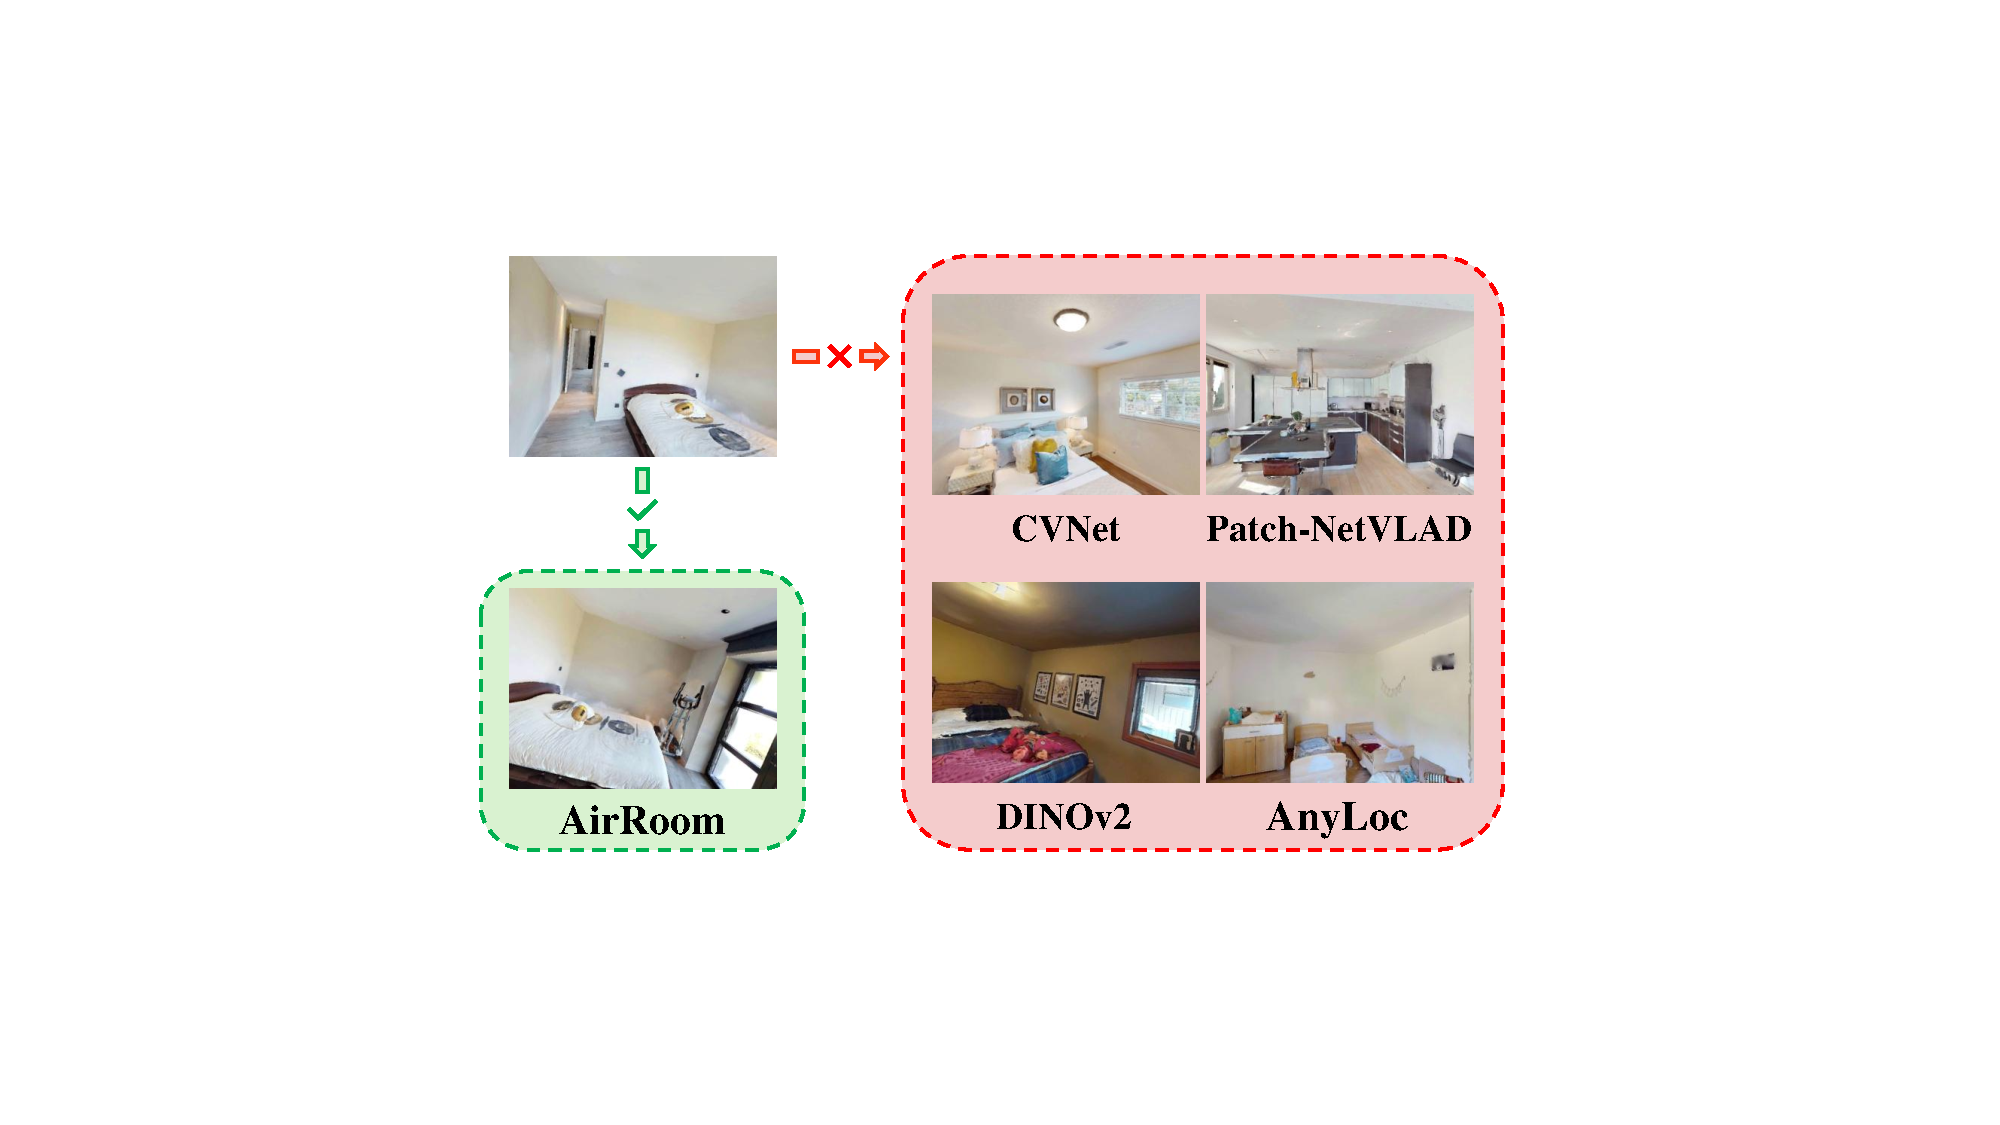
\includegraphics[width=\columnwidth]{failure_font.pdf}
    \vspace{-16pt}
    \caption{Given a bedroom query, AirRoom accurately retrieves the target image by leveraging object relevance for room reidentification. In contrast, CVNet retrieves visually similar images without preserving scene accuracy, DINOv2 captures semantic content but overlooks color details, Patch-NetVLAD, using aggregated local features to form global descriptors, retrieves images with mismatched semantic information, and AnyLoc considers semantic and color attributes but neglects object importance within rooms.}
    \vspace{-5pt}
    \label{fig:failure}
\end{figure}

\tref{tab:overall} presents a quantitative comparison between AirRoom and baseline methods, showing that AirRoom outperforms all baselines on nearly all metrics and datasets. In room reidentification tasks, image retrieval methods generally exhibit lower classification metrics due to their focus not being on top-1 precision, while VPR methods yield better results. Global descriptor-based VPR methods capture only high-level semantic information, often retrieving rooms with similar semantics but lacking detailed features. In contrast, VPR methods using aggregated local features, such as Patch-NetVLAD, emphasize low-level encodings but may overlook global context, resulting in less accurate retrievals. \fref{fig:failure} illustrates failure cases for CVNet, DINOv2, Patch-NetVLAD, and AnyLoc, highlighting these limitations. 
Although AnyLoc, known for its robust performance in ``anywhere, anytime, anyview" VPR, performs well, AirRoom further enhances performance, achieving a 20\% to 40\% improvement within the available margin compared to AnyLoc. For instance, AnyLoc achieves 89.69\% accuracy on HMReID, leaving approximately 10\% room for improvement. AirRoom, with an accuracy of 93.80\%, demonstrates up to a 40\% improvement within this remaining margin. These results highlight AirRoom's superior precision and refinement in room reidentification.

% \vspace{-4pt}
\subsection{Group-Wise Performance Comparison}
\label{sec:section4.5}
\vspace{-3pt}
Many baseline methods adopt a “backbone + enhancement mechanism” paradigm, which our approach also follows. In this section, we compare the performance of our object-aware enhancement mechanism with that of several state-of-the-art methods, using the same backbone as each group’s baseline. This setup allows us to directly assess the effectiveness of our object-aware enhancement mechanism.

For the ResNet50 backbone group, we use CVNet \cite{lee2022correlationverificationimageretrieval} as the baseline. In the NetVLAD backbone group, we employ Patch-NetVLAD \cite{hausler2021patchnetvladmultiscalefusionlocallyglobal} as the baseline, testing it at three reduction dimensions: 4096, 512, and 128.

\tref{tab:grouped} reveals that within each group, the single backbone outperforms the baseline methods that attempt to enhance performance through various mechanisms, indicating that these mechanisms do not effectively capture critical information in indoor rooms. In contrast, our object-aware enhancement mechanism significantly improves the backbone’s performance by emphasizing the importance of \mbox{objects} in indoor environments.

% \vspace{-4pt}
\subsection{Pipeline Flexibility Evaluation}
\label{sec:section4.6}
\vspace{-3pt}
In this section, we systematically evaluate the flexibility and adaptability of AirRoom by testing different configurations of its key modules. The results clearly demonstrate that AirRoom is not reliant on any specific model and can effectively integrate a diverse range of models.

\vspace{-5pt}
\subsubsection{Global Feature Extractor}
\vspace{-4pt}
We test various Global Feature Extractors, including ViT \cite{dosovitskiy2021imageworth16x16words}, DINO \cite{caron2021emergingpropertiesselfsupervisedvision}, DINOv2 \cite{oquab2024dinov2learningrobustvisual}, and AnyLoc-VLAD-DINOv2 \cite{keetha2023anylocuniversalvisualplace} with VLAD cluster sizes of 16 and 8.

As shown in \tref{tab:global feature extractor flexibility}, AirRoom consistently achieves over 85\% across all metrics and datasets in nearly every case, regardless of the capabilities of the Global Feature Extractor used. Even in the single exception with DINOv2, AirRoom still improves performance by nearly 15\%. This demonstrates that the effectiveness of our pipeline is not reliant on any specific Global Feature Extractor, highlighting AirRoom's adaptability to various backbone configurations and underscoring its robust flexibility.


\vspace{-5pt}
\subsubsection{Instance Segmentation}
\vspace{-4pt}
We compare traditional instance segmentation methods, such as Mask R-CNN \cite{he2018maskrcnn}, with more recent approaches, including Semantic-SAM \cite{li2023semanticsamsegmentrecognizegranularity}, which leverage advanced techniques for more granular segmentation.

\tref{tab:is flexibility} shows that AirRoom consistently outperforms the baseline by over 15\%, regardless of the instance segmentation module used. This demonstrates that our pipeline is not dependent on any specific instance segmentation method, underscoring its adaptability in this component.

\begin{table}[h]
\vspace{-5pt}
\centering
\resizebox{\columnwidth}{!}{%
\begin{tabular}{l|cccc}
\toprule
\multirow{2}{*}{\textbf{Methods}} & \multicolumn{4}{c}{\textbf{HMReID}} \\
 & Accuracy & Precision & Recall & F1 \\
\midrule
DINOv2 & 53.91 & 60.52 & 53.73 & 54.69 \\
\rowcolor{Lavender} AirRoom-MaskRCNN & 69.44 & 72.23 & 69.08 & 69.07 \\
\rowcolor{Lavender} AirRoom-SSAM & \textbf{70.95} & \textbf{73.86} & \textbf{70.66} & \textbf{70.78} \\
\bottomrule
\end{tabular}%
}
\vspace{-10pt}
\caption{Instance Segmentation Flexibility.}
\vspace{-16pt}
\label{tab:is flexibility}
\end{table}



\subsubsection{Object Feature Extractor}

We experiment with both traditional backbones, such as ResNet50 \cite{he2015deepresiduallearningimage}, and more modern backbones, like DINOv2 \cite{oquab2024dinov2learningrobustvisual}, as the Object Feature Extractor.

As shown in \tref{tab:ofe flexibility}, AirRoom achieves substantial performance improvements over the baseline, with minimal performance variation between different Object Feature Extractors. This supports the flexibility of our pipeline in accommodating a range of feature extraction methods.

\begin{table}[h]
\vspace{-6pt}
\centering
\resizebox{\columnwidth}{!}{%
\begin{tabular}{l|cccc}
\toprule
\multirow{2}{*}{\textbf{Methods}} & \multicolumn{4}{c}{\textbf{HMReID}} \\
 & Accuracy & Precision & Recall & F1 \\
\midrule
DINOv2 & 53.91 & 60.52 & 53.73 & 54.69 \\
\rowcolor{Lavender} AirRoom-ResNet50 & \textbf{70.95} & \textbf{73.86} & \textbf{70.66} & \textbf{70.78} \\
\rowcolor{Lavender} AirRoom-DINOv2 & 68.67 & 71.81 & 68.33 & 68.59 \\
\bottomrule
\end{tabular}%
}
\vspace{-10pt}
\caption{Object Feature Extractor Flexibility.}
\vspace{-20pt}
\label{tab:ofe flexibility}
\end{table}





\subsubsection{Object-Aware Scoring}

We evaluate both the mean (\(s_{\text{mean}}\)) and max (\(s_{\max}\)) strategies for computing the patch score (\(s_{\text{patch}}\)) and object score (\(s_{\text{object}}\)), assessing their impact on the overall performance.

\tref{tab:os flexibility} shows that AirRoom’s performance remains stable regardless of the object-aware scoring method used. This underscores the robustness of object-oriented information in room reidentification and demonstrates AirRoom’s flexibility in adapting to different scoring strategies.

\begin{table}[h]
\vspace{-6pt}
\centering
\resizebox{\columnwidth}{!}{%
\begin{tabular}{l|cccc}
\toprule
\multirow{2}{*}{\textbf{Methods}} & \multicolumn{4}{c}{\textbf{HMReID}} \\
 & Accuracy & Precision & Recall & F1 \\
\midrule
DINOv2 & 53.91 & 60.52 & 53.73 & 54.69 \\
\rowcolor{Lavender} AirRoom-Max(patch)-Mean(object) & 70.95 & 73.86 & 70.66 & 70.78 \\
\rowcolor{Lavender} AirRoom-Max(patch)-Max(object) & \textbf{71.02} & \textbf{74.02} & \textbf{70.72} & \textbf{70.85} \\
\rowcolor{Lavender} AirRoom-Mean(patch)-Max(object) & 70.85 & 73.85 & 70.55 & 70.70 \\
\rowcolor{Lavender} AirRoom-Mean(patch)-Mean(object) & 70.90 & 73.78 & 70.62 & 70.73 \\
\bottomrule
\end{tabular}%
}
\vspace{-10pt}
\caption{Object-Aware Scoring Flexibility.}
\vspace{-20pt}
\label{tab:os flexibility}
\end{table}


\subsection{Ablation Studies}
\label{sec:section4.7}

In this section, we remove certain modules from our pipeline—including the global score \(s_{\text{global}}\),  the patch score \(s_{\text{patch}}\), the object score \(s_{\text{object}}\), within object-aware scoring, and the entire Fine-Grained Retrieval (FGR)—to assess the importance and effectiveness of each component.

\begin{table}[t]
\centering
\resizebox{\columnwidth}{!}{%
\begin{tabular}{l|cccc}
\toprule
\multirow{2}{*}{\textbf{Methods}} & \multicolumn{4}{c}{\textbf{HMReID}} \\
 & Accuracy & Precision & Recall & F1 \\
\midrule
DINOv2 (AirRoom-w/o all)& 53.91 & 60.52 & 53.73 & 54.69 \\
\rowcolor{Lavender} AirRoom-w/o \(s_{\text{patch}}\) & 66.68 & 70.04 & 66.42 & 66.68 \\
\rowcolor{Lavender} AirRoom-w/o \(s_{\text{object}}\) & 69.77 & 72.84 & 69.48 & 69.64 \\
\rowcolor{Lavender} AirRoom-w/o FGR & 66.11 & 70.85 & 65.80 & 66.41 \\
\rowcolor{Lavender} AirRoom-w/o \(s_{\text{patch}}\) \& \(s_{\text{object}}\) & 62.26 & 66.43 & 62.03 & 62.46 \\
\rowcolor{Lavender} AirRoom-w/o \(s_{\text{patch}}\) \& FGR & 59.39 & 65.25 & 59.14 & 59.97 \\
\rowcolor{Lavender} AirRoom-w/o \(s_{\text{object}}\) \& FGR & 63.44 & 68.68 & 63.14 & 63.84 \\
\rowcolor{Lavender} AirRoom & \textbf{70.95} & \textbf{73.86} & \textbf{70.66} & \textbf{70.78} \\
\bottomrule
\end{tabular}%
}
\vspace{-10pt}
\caption{Ablation Studies (Excluding Global Score Experiments).}
\vspace{-6pt}
\label{tab:ablation w/o global score}
\end{table}

\begin{table}[ht]
\centering
\resizebox{\columnwidth}{!}{%
\begin{tabular}{l|cccc}
\toprule
\multirow{2}{*}{\textbf{Methods}} & \multicolumn{4}{c}{\textbf{HMReID}} \\
 & Accuracy & Precision & Recall & F1 \\
\midrule
ViT & 76.47 & 79.37 & 76.04 & 75.91 \\
\rowcolor{Lavender} AirRoom-ViT-w/o \(s_{\text{global}}\) & 84.86 & 86.82 & 84.34 & 84.61 \\
\rowcolor{Lavender} AirRoom-ViT & \textbf{86.58} & \textbf{88.13} & \textbf{86.12} & \textbf{86.23} \\
\cdashline{1-5}
DINOv2 & 53.91 & 60.52 & 53.73 & 54.69 \\
\rowcolor{Lavender} AirRoom-DINOv2-w/o \(s_{\text{global}}\) & \textbf{71.73} & \textbf{74.97} & \textbf{71.44} & \textbf{71.64} \\
\rowcolor{Lavender} AirRoom-DINOv2 & 70.95 & 73.86 & 70.66 & 70.78 \\
\bottomrule
\end{tabular}%
}
\vspace{-10pt}
\caption{Ablation Studies on Global Score.}
\vspace{-15pt}
\label{tab:ablation on global score}
\end{table}

\tref{tab:ablation w/o global score} shows that removing any module from our pipeline leads to a performance drop. However, as long as at least one module remains, our pipeline still outperforms the baseline. \tref{tab:ablation on global score}  demonstrates that when the Global Feature Extractor (ViT) performs well, the global score \(s_{\text{global}}\) significantly enhances performance. On the other hand, when the Global Feature Extractor (DINOv2) is less effective, the global score \(s_{\text{global}}\) has a slight negative impact, causing a small drop in performance. This result aligns with our hypothesis in Section~\ref{subsec:refinement}, where the global score acts as a prior to rank the priority of the five candidates. Overall, these ablation studies confirm that every module in our pipeline is both important and necessary.

\subsection{Limitations}

While AirRoom achieves state-of-the-art performance in room reidentification under various viewpoint variations, a limitation of our work is the inability to verify robustness to indoor object rearrangements caused by movable objects. Although our mutual nearest neighbors-based Object-Aware Scoring method is somewhat robust to such rearrangements, the datasets used in our experiments lack these cases. In contrast, recent advances in dynamic scene understanding \cite{zhao2024dynamicsceneunderstandingobjectcentric} focus on recognizing scenes in the presence of moving objects, potentially offering greater robustness than our approach. Future work should consider constructing datasets that include object rearrangements and integrating new techniques to enhance robustness to movable objects, thereby improving room reidentification.